\documentclass[../main.tex]{subfiles}

\begin{document}

\begin{questions}

\question Calculate the magnetic force of attraction between the northern and southern hemispheres of a spinning charged magnetic shell (with radius $R$, angular speed $\omega$ and surface charge density $\sigma$)
\begin{solution}
	Let us orient the $z$ axis along $\vec{\omega}$\\ 
	We already know the vector potential
	\begin{align}
		\vec{A}(\vec{r}) &=
		\begin{cases}
			\frac{\mu_0\omega\sigma}{3}r\sin\theta\,\hat{\phi} & r\leq R\\
			\frac{\mu_0\omega R^4\sigma}{3}\frac{\sin\theta}{r^2}\,\hat{\phi} & r\geq R
		\end{cases}
	\end{align}
	We need the $\vec{B}_\text{ave}=\frac{\vec{B}_\text{in}(R) + \vec{B}_\text{out}(R)}{2}$ at the surface of the shell
	\begin{align}
		\vec{B}_\text{in}(R)=\left.\nabla\times\vec{A}_\text{in}\right|_{r=R}&=\frac{2}{3}\mu_0R\omega\sigma\,\hat{z}\\
		\vec{B}_\text{out}(R)  =\left.\nabla\times\vec{A}_\text{out}\right|_{r=R}&=\frac{\mu_0R\omega\sigma}{3}(2\cos\theta\,\hat{r}+\sin\theta\,\hat{\theta})\\
		\implies \vec{B}_\text{ave} &= \frac{\mu_0R\omega\sigma}{6}(4\cos\theta\,\hat{r}-\sin\theta\,\hat{\theta})
	\end{align}
	Now to find the force due to this $\vec{B}$ on the surface current $\vec{K}$\\
	We know that $\vec{K}=\sigma\vec{v}=\omega R\sin\theta\,\hat{\phi}$
	\begin{align}
		\vec{K}\times\vec{B}_\text{ave} &= \frac{\mu_0}{6}\sin\theta(\sigma\omega R)^2(4\cos\theta\,\hat{\theta}+\sin\theta\,\hat{r})
	\end{align}
	Finally,
	\begin{align}
		\vec{F} &= \int_\mathcal{S}\vec{K}\times\vec{B}_\text{ave}\,dA\\
		\intertext{Only the $z$ component will survive the integral}
		\vec{F} &= -\frac{\mu_0}{2}(\sigma\omega R^2)R^2\,\hat{z}\int_{\phi=0}^{2\pi}\int_{\theta=0}^{\frac{\pi}{2}}\sin^3\theta\cos\theta\,d\theta\,d\phi = -\frac{\mu_0\pi}{4}(\sigma\omega R^2)^2\,\hat{z}
	\end{align}
\end{solution}
	
\question What current density would produce the vector potential, A = k$\hat{\phi}$ (where k is a constant), in cylindrical coordinates?
\begin{solution}
Given $A_{\phi}=k$, so using $B=\nabla\times A$, in cylindrical coordinates, we get $B = \frac{k}{s}\hat{z}$.\\
Next, by using $J=\frac{\nabla\times B}{\mu_0}$, in cylindrical coordinates, we get $J=\frac{k}{\mu_0 s^2}\hat{\phi}$.
\end{solution}
	
\question A sphere of radius $R$ carries a polarization
P(r) = $k$r where $k$ is a constant and r is the vector from the center.

\begin{parts}
	\part Calculate the bound charges $\sigma_b$ and $\rho_b$
	\begin{solution}
$\sigma_b=P.\hat{n}=kR$, $\rho_b=-\nabla.P=-3k$
	\end{solution}

	\part Find the electric field inside and outside the sphere.
	\begin{solution}
Inside the sphere, $E=\frac{\rho r}{3\epsilon_0}\hat{r}$, so using $\rho$, we get $E=\frac{-k}{\epsilon_0}r$\\
For calculating E outside the sphere, we can use the fact that the net charge at the center is 0, so effectively E=0.
	\end{solution}
\end{parts}
	
\question A thick spherical shell having inner radius $a$ and outer radius $b$ is made of dielectric material with a ``frozen-in" polarization $\textbf{P(r)}=\frac{k}{r}\hat{r}$ where $k$ is a constant and $r$ is the distance from the center and no free charge is present, then find D and E for all 3 regions. Refer Figure \ref{fig:f1}.

\begin{figure}[H]
	\centering
	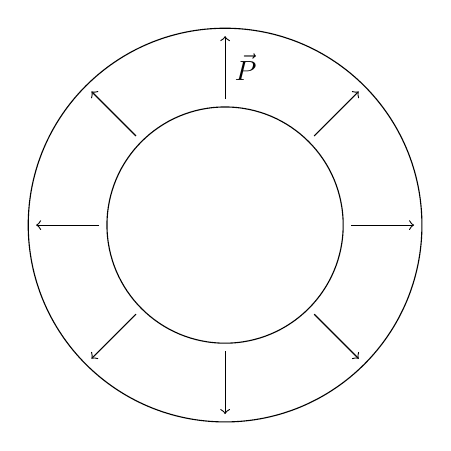
\begin{tikzpicture}
		\draw (0,0) circle (1.5);
		\draw (0,0) circle (2.5);

		\foreach \x in {1,...,8}
		{
			\draw[->] ({1.6*cos(\x*45)},{1.6*sin(\x*45)}) -- ({2.4*cos(\x*45)},{2.4*sin(\x*45)});
		}

		\node at (0,2) [right]{$\vec{P}$};
	\end{tikzpicture}
	\caption{Shell with $\vec{P}(\vec{r})$}
	\label{fig:f1}
\end{figure}


\begin{solution}
Since no free charge is present so D=0 everywhere.\\
By using $D=\epsilon_0E +P$, we get $E=-\frac{1}{\epsilon_0}P$, So $E\neq0$ only for $a<r<b$ in which case we get $E=\frac{-k}{\epsilon_0r}\hat{r}$. For $r<a, r>b$ the net charge is 0, hence E=0.
\end{solution}
	
\question In the lecture, we have calculated the total field inside the sphere when a sphere made of homogeneous linear isotropic dielectric (with dielectric constant $\epsilon_r$) material is placed in an otherwise uniform electric field $\vec{E}_0$ by solving Laplace's equation:
\begin{equation*}
	\vec{E} = \frac{3}{\epsilon_r + 2}E_0
\end{equation*}
Attempt an alternate (and possibly more intuitive) approach to this, as follows. First find the polarization $\vec{P_0}$ due to $\vec{E_0}$. This polarization generates a field of its own, $\vec{E_1}$ which in turns causes an additional polarization $\vec{P_1}$, which further generates an additional field $\vec{E_2}$ and so on. Show that resultant field inside the sphere $\vec{E} = \vec{E_0} + \vec{E_1} + \vec{E_2} + \dots$ matches that what we get by solving Laplace's Equation.
\begin{solution}
	We know that
	\begin{align}
		\vec{P}_i &= \chi_e\epsilon_0\vec{E_i} = (\epsilon_r-1)\epsilon_0\vec{E}_i
	\end{align}
	We also have
	\begin{align}
		\vec{P}_{i+1} &= -\frac{1}{3\epsilon_0}\vec{E}_i
	\end{align}
	Thus we end up with
	\begin{align}
		\vec{E}_i &= \left(-\frac{\epsilon_r-1}{3}\right)^i\vec{E}_0\\
		\implies \vec{E} = \sum_{i=0}^{\infty} \vec{E_i} &= \frac{3}{\epsilon_r + 2}\vec{E}_0
	\end{align}
\end{solution}

\question Find the electric potential inside and outside a homogeneous linear isotropic dielectric sphere (with dielectric constant $\epsilon_r$ and radius $R$), at the centre of which a pure dipole $\vec{p}$ is imbedded.
\begin{solution}
	We will find solution's to Laplace's equation in the region $r < R$ (excluding a small region containing the dipole), and $r>R$ separately.\\ Using separation of variables,
	\begin{align}
		V_\text{in}(r,\theta) &= \sum_{l=0}^{\infty} \left(A^\text{(in)}_lr^l+\frac{B^\text{(in)}_l}{r^{l+1}}\right)P_l(\cos\theta)\\
		V_\text{out}(r,\theta) &= \sum_{l=0}^{\infty} \left(A^\text{(out)}_lr^l+\frac{B^\text{(out)}_l}{r^{l+1}}\right)P_l(\cos\theta)
	\end{align}
	Subject to boundary conditions
	\begin{align}
		\lim_{r\to\infty}V_\text{out}(r,\theta) &= 0\label{eq:9bc1}
		\\
		\lim_{r\to0}V_\text{in}(r,\theta) &= \frac{1}{4\pi\epsilon_0\epsilon_r} \frac{p\cos\theta}{r^2}\label{eq:9bc2}
		\\
		V_\text{in}(R,\theta) &= V_\text{out}(R,\theta)\label{eq:9bc3} && \text{$\because \text{ }$ continuity of $V$}
		\\
		\epsilon_0\epsilon_r\left.\frac{\partial V_\text{in}}{\partial r}\right|_{r=R} &= \epsilon_0\left.\frac{\partial V_\text{out}}{\partial r}\right|_{r=R}  && \because \text{ } D^{\perp}_\text{out} - D^{\perp}_\text{in} = \sigma_f = 0 \label{eq:9bc4}
	\end{align}
	Applying \eqref{eq:9bc1} and \eqref{eq:9bc2} we can immediately see that $A^\text{(out)}_l=0$ $\forall$ $l$; $B^\text{(in)}_l=0$ $\forall$ $l\neq1$; $B^\text{(in)}_1 = \frac{p}{4\pi\epsilon_0\epsilon_r}$\\
	Applying \eqref{eq:9bc3} and \eqref{eq:9bc4},
	\begin{align}
		A^\text{(in)}_l &= 0 \text{ } \forall \text{ } l \neq 1\\
		B^\text{(out)}_l &= 0 \text{ } \forall \text{ } l \neq 1\\
		A_1^\text{(in)}R+\frac{p}{4\pi\epsilon_0\epsilon_rR^2} &= \frac{B_1^\text{(out)}}{R^2}\\
		\epsilon_rA_1^\text{(in)} - \frac{2p}{4\pi\epsilon_0R^3} &= \frac{-2B_1^\text{(out)}}{R^3}
	\end{align}
	Solving,
	\begin{align}
		B^\text{(out)} &= \frac{p}{4\pi\epsilon_0}\frac{3}{\epsilon_r+2}\\
		A^\text{(in)} &= \frac{p}{4\pi\epsilon_0R^3}\frac{2(\epsilon_r-1)}{\epsilon_r(\epsilon_r+2)}        
	\end{align}
	Thus we finally have,
	\begin{align}
		V_\text{in}(r,\theta) &= \frac{p\cos\theta}{4\pi\epsilon_0\epsilon_rr^2}\left(1 + \frac{r^3}{R^3}\frac{2(\epsilon_r-1)}{\epsilon_r+2}\right)\\
		V_\text{out}(r,\theta) &= \frac{p\cos\theta}{4\pi\epsilon_0 r^2}\frac{3}{\epsilon_r+2}
	\end{align}
\end{solution}
	
\question A cylinder of radius R and height L is positioned such that the origin is at the center and the z-axis is along the axis of the cylinder. The cylinder carries a frozen polarisation $\vec{P} = {P_o}\hat{z}$. Calculate $\vec{E}$ and $\vec{D}$ at all points on the z-axis. Are the quantities $\vec{D}$ and $\vec{E}$ proportional to each other inside the material?

\begin{solution}
	Since $\vec{P}$ is uniform, the bound volume charge density is $-\nabla\cdot\vec{P}=0$. There exists only a uniform bound surface charge density at the ends of the bar electret, $\sigma=\vec{P}\cdot\hat{n}=\pm P_0$

	Therefore the only $\vec{E}$ field is due to the two discs of radius $\vec{R}$, parallel to $xy$ plane and centered at $(0,0,\pm\frac{L}{2})$, and having uniform surface charge density $P_0$ and $-P_0$
	\begin{figure}[H]
		\centering
		\begin{tikzpicture}
			\draw (0,0) rectangle (3,5);

			\begin{scope}[very thick,decoration={
				markings,
				mark=at position 0.4 with {\arrow{Latex}},
				mark=at position 0.7 with {\arrow{Latex}}}
				]

				\foreach \y in {-4,...,4}
				{
					\draw[postaction={decorate}] plot [smooth] coordinates {({1.5+0.3*\y},5) ({1.5+0.35*\y},4) ({1.5+0.6*\y},2.5) ({1.5+0.35*\y},1) ({1.5+0.3*\y},0)};
				}

			\end{scope}

			\begin{scope}[very thick,decoration={
				markings,
				mark=at position 0.8 with {\arrow{Latex}}
				}]

				\draw[postaction={decorate}] plot [smooth] coordinates { ({1.5+2/3},5) ({1.5+2/3+0.1},6) ({1.5+2/3+0.3},7) };
				\draw[postaction={decorate}] plot [smooth] coordinates { ({1.5+2/3+0.3},-2) ({1.5+2/3+0.1},-1) ({1.5+2/3},0) };
				\draw[postaction={decorate}] plot [smooth] coordinates { ({1.5-2/3},5) ({1.5-2/3-0.1},6) ({1.5-2/3-0.3},7) };
				\draw[postaction={decorate}] plot [smooth] coordinates { ({1.5-2/3-0.3},-2) ({1.5-2/3-0.1},-1) ({1.5-2/3},0)};

				\draw[postaction={decorate}] (1.5,5) -- (1.5,7);
				\draw[postaction={decorate}] (1.5,-2) -- (1.5,0);

			\end{scope}

			\begin{scope}[very thick,decoration={
				markings,
				mark=at position 0.3 with {\arrow{Latex}},
				mark=at position 0.8 with {\arrow{Latex}},
				}]
				\path[clip] (3,2.5) -- (3,5) -- (1.5,5) -- (1.5,7) -- (5.5,7) -- (5.5,-2) -- (1.5,-2) -- (1.5,0) -- (3,0) -- cycle;

				\draw[postaction={decorate}] plot[smooth cycle] coordinates { ({1.5+2/3+0.3},2.5) ({1.5+4.3/3},5.1) ({1.5+3.7},2.5) ({1.5+4.3/3},-0.1) };
			\end{scope}

			\begin{scope}[very thick,decoration={
				markings,
				mark=at position 0.3 with {\arrow{Latex}},
				mark=at position 0.8 with {\arrow{Latex}},
				}]
				\path[clip] (0,2.5) -- (0,5) -- (1.5,5) -- (1.5,7) -- (-2.5,7) -- (-2.5,-2) -- (1.5,-2) -- (1.5,0) -- (0,0) -- cycle;

				\draw[postaction={decorate}] plot[smooth cycle] coordinates { ({1.5-2/3-0.3},2.5) ({1.5-4.3/3},5.1) ({1.5-3.7},2.5) ({1.5-4.3/3},-0.1) };
			\end{scope}

		\end{tikzpicture}
		\caption{$\vec{E}$ field for the bar electret}
	\end{figure}

	This $\vec{E}$ field is obviously curl-less and suffers from discontinuities at the electret ends owing to the surface (bound) charges

	We can find the $\vec{E}$ field on the z axis quantitatively since we know the field on the axis of a disc
	\begin{align}
		\vec{E} &= 
		\begin{cases}
			-\frac{P_0}{2\epsilon_0}\left(2-\frac{\frac{L}{2}-z}{\sqrt{(\frac{L}{2}-z)^2+R^2}}-\frac{\frac{L}{2}+z}{\sqrt{(\frac{L}{2}+z)^2+R^2}}\,\right)\,\khat & -\frac{L}{2} < z < \frac{L}{2}\\
			\frac{P_0}{2\epsilon_0}\left(\frac{\frac{L}{2}+z}{\sqrt{(\frac{L}{2}+z)^2+R^2}}-\frac{z-\frac{L}{2}}{\sqrt{(z-\frac{L}{2})^2+R^2}}\right)\,\khat & z > \frac{L}{2}\\
			\frac{P_0}{2\epsilon_0}\left(\frac{\frac{L}{2}-z}{\sqrt{(\frac{L}{2}-z)^2+R^2}}-\frac{-z-\frac{L}{2}}{\sqrt{(\frac{L}{2}+z)^2+R^2}}\right)\,\khat & z < -\frac{L}{2}
		\end{cases}\\
		\intertext{We can thus find $\vec{D}$}
		\vec{D} = \epsilon_0\vec{E} + \vec{P} &= 
		\begin{cases}
			\frac{P_0}{2}\left(\frac{\frac{L}{2}-z}{\sqrt{(\frac{L}{2}-z)^2+R^2}}+\frac{\frac{L}{2}+z}{\sqrt{(\frac{L}{2}+z)^2+R^2}}\,\right)\,\khat & -\frac{L}{2} < z < \frac{L}{2}\\
			\frac{P_0}{2}\left(\frac{\frac{L}{2}+z}{\sqrt{(\frac{L}{2}+z)^2+R^2}}-\frac{z-\frac{L}{2}}{\sqrt{(z-\frac{L}{2})^2+R^2}}\right)\,\khat & z > \frac{L}{2}\\
			\frac{P_0}{2}\left(\frac{\frac{L}{2}-z}{\sqrt{(\frac{L}{2}-z)^2+R^2}}-\frac{-z-\frac{L}{2}}{\sqrt{(\frac{L}{2}+z)^2+R^2}}\right)\,\khat & z < -\frac{L}{2}
		\end{cases}\\
		&=\frac{P_0}{2}\left(\frac{\frac{L}{2}-z}{\sqrt{(\frac{L}{2}-z)^2+R^2}}+\frac{\frac{L}{2}+z}{\sqrt{(\frac{L}{2}+z)^2+R^2}}\,\right)\,\khat
	\end{align}

	$\vec{D}$ is of course only $\propto\vec{E}$ outside the electret

	\begin{figure}[H]
		\centering

		\begin{tikzpicture}
			\draw (0,0) rectangle (3,5);

			\begin{scope}[very thick,decoration={
				markings,
				mark=at position 0.5 with {\arrow{Latex}}
				}]

				\draw[postaction={decorate}] plot [smooth] coordinates { ({1.5+2/3+0.3},-2) ({1.5+2/3+0.1},-1) ({1.5+2/3},0) ({1.5+2/3-0.1},2.5) ({1.5+2/3},5) ({1.5+2/3+0.1},6) ({1.5+2/3+0.3},7) };

				\draw[postaction={decorate}] plot [smooth] coordinates { ({1.5-2/3-0.3},-2) ({1.5-2/3-0.1},-1) ({1.5-2/3},0) ({1.5-2/3+0.1},2.5) ({1.5-2/3},5) ({1.5-2/3-0.1},6) ({1.5-2/3-0.3},7) };

				\draw[postaction={decorate}] (1.5,-2) -- (1.5,5) -- (1.5,7);

			\end{scope}

			% \begin{scope}[very thick,decoration={
			% 	markings,
			% 	mark=at position 0.3 with {\arrow{Latex}},
			% 	mark=at position 0.8 with {\arrow{Latex}},
			% 	}]

			% 	\draw[postaction={decorate}] plot [smooth cycle] coordinates { ({1.5+4/3},5) ({1.5+4.5/3},5.3) ({1.5+5.5/3},5.3) ({1.5+2.4},5) ({1.5+3.55},4) ({1.5+4.5},2.5) ({1.5+3.55},1) ({1.5+2.4},0) ({1.5+5.5/3},-0.3) ({1.5+4.5/3},-0.3) ({1.5+4/3},0) ({1.5+4/3-0.3},2.5) ({1.5+4/3},5)};
			% 	\draw[postaction={decorate}] plot [smooth] coordinates { ({1.5-4/3},5) ({1.5-4.5/3},5.3) ({1.5-5.5/3},5.3) ({1.5-2.4},5) ({1.5-3.55},4) ({1.5-4.5},2.5) ({1.5-3.55},1) ({1.5-2.4},0) ({1.5-5.5/3},-0.3) ({1.5-4.5/3},-0.3) ({1.5-4/3},0)};

			% \end{scope}

			\begin{scope}[very thick,decoration={
					markings,
					mark=at position 0.3 with {\arrow{Latex}},
					mark=at position 0.8 with {\arrow{Latex}},
					}]

				\draw[postaction={decorate}] plot[smooth cycle] coordinates { ({1.5+2/3+0.3},2.5) ({1.5+4.3/3},5.1) ({1.5+3.7},2.5) ({1.5+4.3/3},-0.1) };

				\draw[postaction={decorate}] plot[smooth cycle] coordinates { ({1.5-2/3-0.3},2.5) ({1.5-4.3/3},5.1) ({1.5-3.7},2.5) ({1.5-4.3/3},-0.1) };
			\end{scope}
			
			
		\end{tikzpicture}
		\caption{$\vec{D}$ field for the bar electret}
	\end{figure}

	This $\vec{D}$ field has no discontinuities, but is not curl-less (it's curl is non-zero at the curved surface of electret and is equal to the curl of $\vec{P}$)

	This is a clear demonstration that there is no analog of Coulomb's law for $\vec{D}$ and $\rho_f$, as $\rho_f=0$ everywhere, yet $\vec{D}\neq 0$
\end{solution}

\question A conducting sphere of radius $R$ is half submerged in a linear, homogeneous, semi-infinite liquid dielectric medium of dielectric constant $\kappa$. The sphere is at a potential $V_0$. Assuming there is no bound charge at the liquid-air interface, calculate

\begin{parts}
	\part the potential at a point outside the sphere
	\begin{solution}
		We begin by noticing that the problem has azimuthal symmetry. We also know that the potential must be continous across the surface of the dielectric medium.\\
		We can intuitively begin by trying a radially symmetric solution. If our potential has no dependance on $\theta$, then it's dependence on $r$ must be $\propto \frac{1}{r}$ by separation of variables technique\\ $\therefore$ $V(\vec{r})=\frac{V_0R}{r}$\\
		We can immediately see that this satisfies our boundary conditions, and also Laplace's equations in the regions of interest, therefore by appealing to Uniqueness theorem, this must be the solution
		\\
		\textbf{Alternate Solution:}\\
		We can try a more rigorous approach to this situation, by dividing up space into 2 regions, $z\geq0$ and $z\leq0$ (both cases $r\geq R$), and finding solutions of Laplace's equation in each region. Thus,
		\begin{align}
			V(r,\theta) &= 
			\begin{cases}
				V_{z^+} & z \geq 0\\
				V_{z^-} & z \leq 0
			\end{cases}
			\\
			V_{z^+}(r,\theta) &= \sum_{l=0}^{\infty} \left(A_l^+r^l + \frac{B_l^+}{r^{l+1}}\right)P_l(\cos\theta)
			\\
			V_{z^-}(r,\theta) &= \sum_{l=0}^{\infty} \left(A_l^-r^l + \frac{B_l^-}{r^{l+1}}\right)P_l(\cos\theta)
			\\
			\lim_{r\to\infty}V_z^+(r,\theta) &= \lim_{r\to\infty}V_z^-(r,\theta) = 0\label{eq:8bc1}
			\\
			V_{z^-}(r,\frac{\pi}{2}) &= V_{z^+}(r,\frac{\pi}{2})\label{eq:8bc2}
			\\
			\kappa\left.\frac{\partial V_{z^-}(r,\theta)}{\partial \theta}\right|_{\theta=\frac{\pi}{2}} &= \left.\frac{\partial V_{z^+}(r,\theta)}{\partial \theta}\right|_{\theta=\frac{\pi}{2}}\label{eq:8bc3}
			\\
			V_{z^+}(R,\theta) &= V_{z^-}(R,\theta)\label{eq:8bc4}
		\end{align}
		Applying \eqref{eq:8bc1}, we can see that $A_l^+ = A_l^- = 0$ $\forall$ $l$\\
		Applying \eqref{eq:8bc2}, we can see that $B_l^+ = B_l^-$ $\forall$ even $l$, and from \eqref{eq:8bc3}, we get that $B_l^+ = \kappa B_l^-$ $\forall$ odd $l$\\
		We can also enforce from \eqref{eq:8bc4} the fact that potential at $R$ is a constant to get $B^l+=B^l-=0$ $\forall$ $l\neq0$\\
		Finally from \eqref{eq:8bc4}, $V(r,\theta) = \frac{V_0R}{r}$
	\end{solution}

	\part the electric field, the electric displacement, and the surface and volume bound charge density in the dielectric
	\begin{solution}
		Let $z<0$ be the region of dielectric, with the sphere centered at origin.
		\begin{align}
			\vec{E}=-\nabla V &= \boxed{V_0 \frac{R}{r^2}\,\hat{r}}
			\\
			\implies \vec{D} = \epsilon\vec{E} &= 
			\boxed{
				\begin{cases}
					\epsilon_0V_0\frac{R}{r^2}\,\hat{r} & z \geq 0\\
					\epsilon_0\kappa V_0\frac{R}{r^2}\,\hat{r} & z \leq 0
				\end{cases}
			}
			\\
			\implies \vec{P} = \chi_e\epsilon_0\vec{E} &=
			\begin{cases}
				0 & z \geq 0\\
				(\kappa-1)\epsilon_0V_0\frac{R}{r^2}\,\hat{r} & z \leq 0
			\end{cases}
			\\
			{\sigma_b}(r=R) = -\vec{P}\cdot\hat{r} &=
			\boxed{
			\begin{cases}
				0 & z \geq 0\\
				(1-\kappa)\epsilon_0V_0\frac{1}{R} & z \leq 0
			\end{cases}
			}
			\\
			{\sigma_b}(z=0) = \vec{P}\cdot\hat{z} &= \boxed{0}
			\\
			\rho_b = -\frac{\chi_e}{1+\chi_e} \rho_f &= \boxed{0}
		\end{align}
	\end{solution}

	\part the total free charge on the conductor.
	\begin{solution}
		We can use Gauss law on a spherical Gaussian surface with $r>R$
		\\
		\begin{align}
			\int_\mathcal{S} \vec{D}\cdot\hat{r} &= Q_f\\
			\implies Q_f &= 2\pi\epsilon_0V_0(1+\kappa)R
		\end{align}
	\end{solution}

\end{parts}

\end{questions}

\end{document}